\chapter{Theoretical  Motivation}

In order to talk about my thesis work it will be necessary to dive into some of the theoretical
background motivating my results. Particle physics is a study of the fundamental building blocks
of the universe and is vast in its nature. I will try to elucidate some of the more pertinent points here. 
I will begin with a brief tour through the Standard Model (SM) followed by a more detailed explanation of
the Higgs mechanism and electroweak symmetry breaking. This chapter was structurally inspired by the 
material in Modern Particle Physics by Mark Thomson \cite{thomson-particle-physics}, which served as 
a steady guide for me throughout my journey in graduate school.

\section{Fundamentals of the Standard Model}

The Standard Model (SM) is a quantum field theory describing all known fundamental particles and 
their interactions through 3 out of the 4 known fundamental forces: the electromagnetic (EM) force, the 
weak nuclear force and the strong nuclear force. It combines our understanding of quantum mechanics and 
special relativity, providing a comprehensive but not completely unified prescription of particle physics 
due to its missing incorporation of general relativity, and thus gravity. The Standard Model 
is defined by its gauge symmetry group $SU(3)\times SU(2)\times U(1)$, which describes a series of local 
mathematical transformations that leave a system of particles invariant. This symmetry is deeply linked with the 
appearance of the three forces incorporated in the SM. In particular, $SU(3)$ is associated with the strong 
nuclear force while $SU(2)\times U(1)$ describes the unified electroweak interaction. The latter symmetry is 
spontaneously broken by the Higgs mechanism, leading to the separate manifestation of the weak and 
EM forces in nature. This mechanism provides the theoretical backbone for my research and will be built up 
throughout this chapter, starting from the basics. The focus of my treatment of the material lies in the symmetries 
themselves, which provide the mathematical foundation for all of the physics we observe.

\subsection{Particles of the Standard Model}

The particles of the SM are broadly grouped into two categories based on their spin: fermions have half-integer 
spin and obey Fermi-Dirac statistics \cite{dirac-fd-statistics} while bosons have integer spin and 
obey Bose-Einstein statistics \cite{bose-be-statistics}. All fundamental fermions in the SM have 
spin-\nicefrac{1}{2} and are further categorized as either quarks or leptons, which make up the matter particles. 
In addition, SM fermions come in 3 generations, each of which consisting of one up-type quark ($q=\frac{2}{3}$), 
one down-type quark ($q=-\frac{1}{3}$), one charged lepton ($q=1$) and one neutrino ($q=0$). Particles in 
successive generations differ only in their masses, making second and third generation fermions inherently 
unstable as they tend to decay into their lighter counterparts. For this reason most ordinary matter in the 
universe is made up of up-quarks, down-quarks and electrons rather than charm-quarks, strange-quarks 
and muons or top-quarks, bottom-quarks and taus. \par

In addition to electromagnetic charge, quarks also have a property called color charge associated with the 
$SU(3)$ symmetry, which enables them to interact via the strong force. Leptons do not possess color charge, 
so they can only interact through the EM \footnote{Only charged particles interact electromagnetically, so this 
does not apply to neutrinos} or weak forces. The latter is the only fundamental interaction that all known particles 
can experience (with some caveats to be discussed in a later section) and is related to the weak isospin $I_3$. 
Alongside the weak hypercharge $Y_W$, $I_3$ is the charge associated with the combined $SU(2) \times U(1)$ 
symmetry corresponding to the electroweak interaction, which is related to EM charge as 
$Q = I_3 + \frac{1}{2}Y_W$. After symmetry breaking, only $Q$ remains conserved universally. Finally, each 
fermion has an anti-particle counterpart with identical characteristics, but opposite EM charge. Since neutrinos 
are charge neutral, their anti-particles are distinguished by their allowed interactions. Currently, it is not clear 
whether neutrinos are their own anti-particles or if anti-neutrinos are fundamentally distinct 
\cite{avignone-majorana-neutrinos}.\par

Bosons in the SM are split into four vector bosons (with spin $s=1$) and one scalar boson (with spin $s=0$): 
the Higgs. Vector bosons are force mediators generated by the symmetry groups of the SM. Gluons are 
associated with the strong force and come in 8 configurations of color charge (associated with the 8 
generators of $SU(3)$). Due to the aforementioned symmetry breaking of $SU(2)\times U(1)$ associated with 
the separation of the weak and EM forces, the photon and $W$ and $Z$ bosons do not map quite as neatly 
onto the generators of this group. In practice, the photon is associated with the EM interaction while the massive 
$W$ and $Z$ bosons propagate the weak interaction. The observation that the mediators of the weak interaction 
are not massless lead to the introduction of a corrective mechanism to the SM which will be described in detail in 
a later section. This is the theoretical origin of the final particle in the SM which is the protagonist of this thesis, 
the Higgs boson. The only known fundamental scalar particle is deeply connected to the existence of particle 
masses and is, for now, the least understood aspect of the Standard Model of particle physics.

%https://www.researchgate.net/figure/The-Standard-Model-of-particle-physics-3_fig1_381551014
\begin{figure}
\centering
    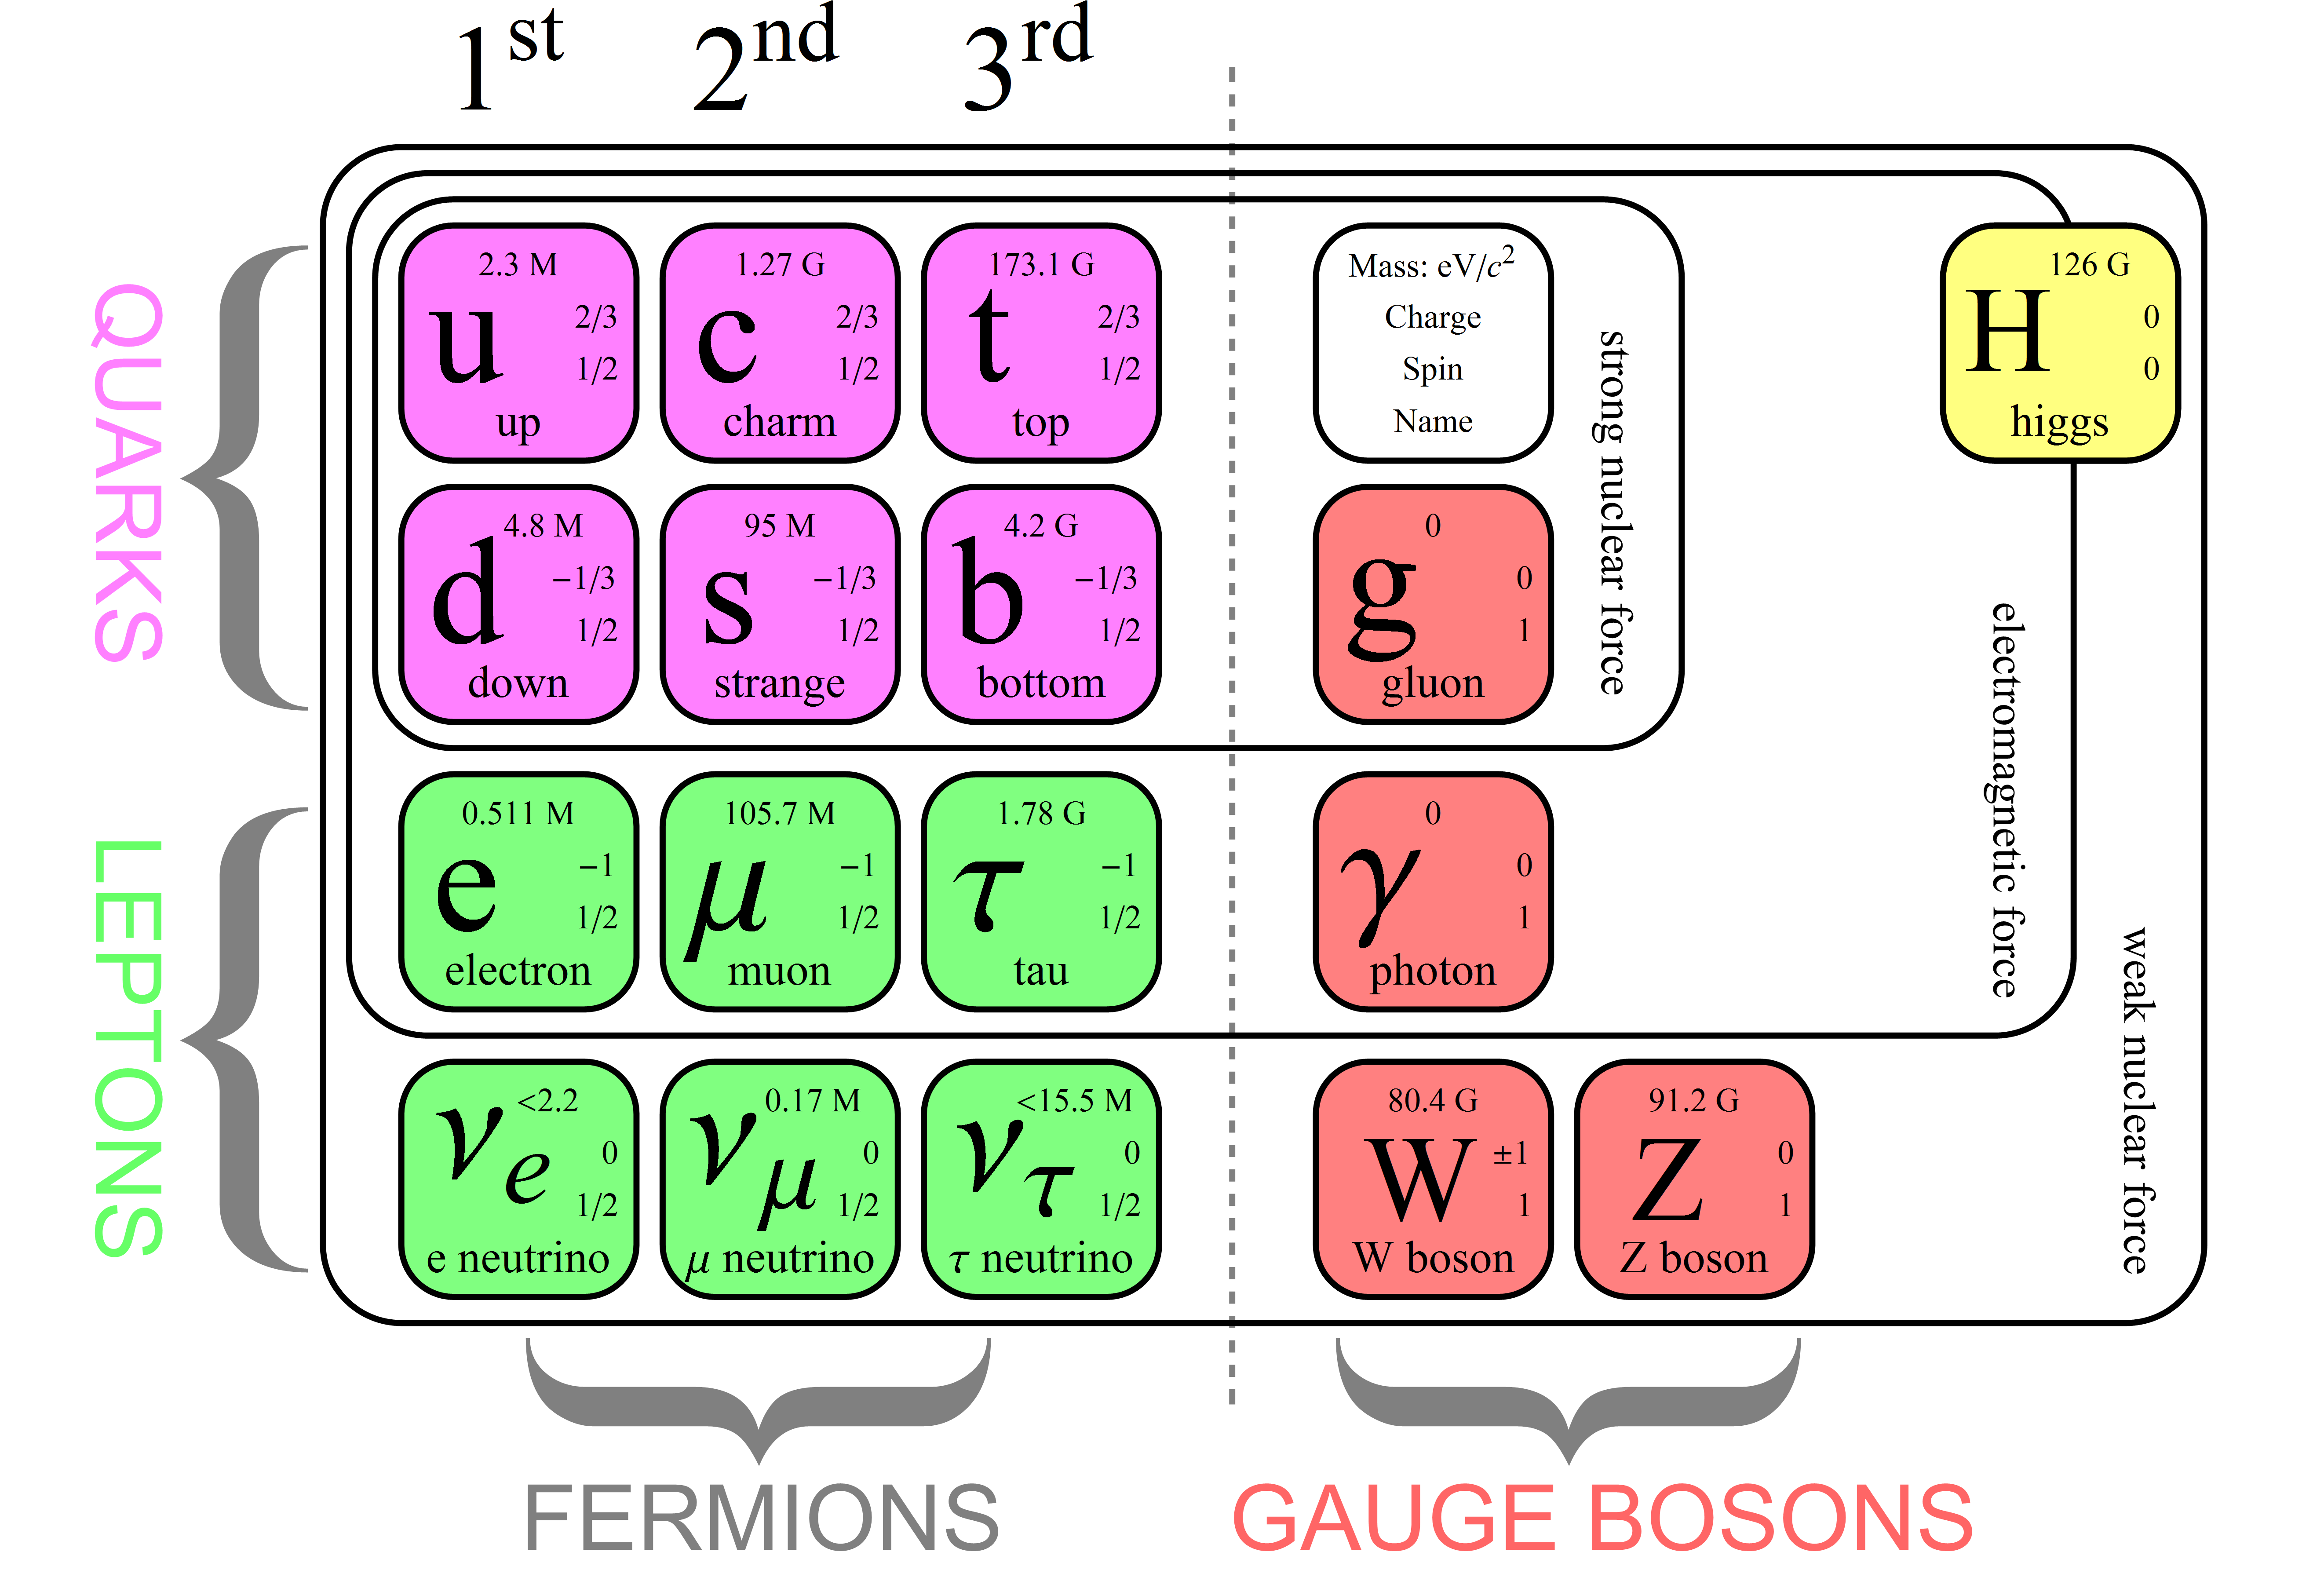
\includegraphics[width=0.8\textwidth]{images/Standard_Model.png}
    \caption{Graphical summary of Standard Model particles.}
    \label{fig:Standard_Model}
\end{figure}

\subsection{Mathematical Formalism}

In order to fully explore the significance of the Higgs boson, a tour through the mathematical formalism of the 
SM is necessary. As a quantum field theory, the fundamental objects of the SM are quantum fields (represented 
by spinors) whose excitations correspond to observable particles. Its Lagrangian $\mathcal{L}_{SM}$ is defined 
by some underlying symmetries, which consist of a global CPT-symmetry in addition to the 
$SU(3)\times SU(2)\times U(1)$ local gauge symmetries discussed above. CPT is a combination of charge 
conjugation (exchange of particles with anti-particles), parity (reversal of space) and time reversal. These three 
symmetries do not always hold individually within the SM (as we will explore), but their combination must always 
remain unbroken. \par

Mathematically, fermions are represented by Dirac spinors $\psi$ which have 4 independent components. 
These can be decomposed into two orthogonal two-component spinors $\psi_L = \frac{1}{2}(1-\gamma_5)\psi$ 
and $\psi_R = \frac{1}{2}(1+\gamma_5)\psi$ which represent chiral eigenstates that are related to each other 
via a parity transformation. This particular decomposition is important because these eigenstates (left-handed 
and right-handed spinors) are treated differently within some SM interactions (leading to violation of 
parity-symmetry). Each chiral spinor has a spin-up and a spin-down component. In the free particle case, a 
fermion field satisfies the Dirac equation 

\begin{equation}
(i\slashed{\partial} - m)\psi = 0
\end{equation}

where $\slashed{\partial} = (i\gamma^{\mu}\partial_{\mu} - m)$. Given $\bar{\psi} = \psi^{\dag}\gamma_0$, 
the free particle Lagrangian then consists simply of a kinetic term and a mass term

\begin{equation}
\mathcal{L} = i\bar{\psi}\gamma^{\mu}\partial_{\mu}\psi - m\bar{\psi}\psi
\end{equation}

This simple picture is complicated significantly by the presence of boson fields, which are responsible for 
introducing particle interactions described by Quantum Electrodynamics (QED), Quantum Chromodynamics 
(QCD), electroweak theory and the Higgs mechanism. Each of these aspects of the SM comes out of a particular 
gauge symmetry or the breaking thereof, which is explored from a mathematical standpoint in the following 
sections.

\subsection{Quantum Electrodynamics (QED)}

Quantum electrodynamics (QED) is the quantum description of electrodynamics, which is one of the oldest 
components of classical physics and describes electricity and magnetism via the electromagnetic force. The 
quantum theory that leads to these classical phenomena postulates that the SM Lagrangian is invariant under a 
$U(1)$ local phase transformation of the form 

\begin{equation}
\psi(x) \rightarrow \psi'(x) = e^{iq\chi(x)}\psi(x)
\end{equation}

This symmetry is enforced with the introduction of the covariant derivative $D_{\mu} = \partial_{\mu} + iqA_{mu}$, 
where $A_{\mu} \rightarrow A_{\mu}' = A_{\mu} + \partial_{\mu}\chi(x)$. The Dirac Lagrangian is thus left invariant 
under the $U(1)$ transformation with the introduction of a new field $A_{\mu}$, which is coupled via the electric 
charge $q$ (and represents the photon). The choice of $\chi(x)$ is arbitrary and leads to the ability to define 
different gauges. This allows for some redundancy in the field description of electrodynamics, which is familiar from 
the classical theory. In practice the $U(1)$ symmetry manifests via the exchange of photons between charged 
particles, described in full by the QED Lagrangian

\begin{equation}
\mathcal{L}_{QED} = - \frac{1}{4}F_{\mu\nu}F^{\mu\nu} + i\bar{\psi}\gamma^{\mu}D_{\mu}\psi - m\bar{\psi}\psi =
- \frac{1}{4}F_{\mu\nu}F^{\mu\nu} + i\bar{\psi}\gamma^{\mu}\partial_{\mu}\psi - q\bar{\psi}\gamma^{\mu}A_{\mu}\psi - m\bar{\psi}\psi
\end{equation}

Here $F_{\mu\nu} = \partial_{\mu}A_{\nu}  - \partial_{\nu}A_{\mu}$ is just the field strength tensor that represents 
the kinetic term of the photon, which describes the propagation of electromagnetic fields. The covariant derivative 
brings out both the standard kinetic term for fermions, as well as a fermion-photon interaction term which is only 
present when $q \neq 0$ as expected. This is the reason photons interact only with particles that carry EM charge.

\subsection{Quantum Chromodynamics (QCD)}

From the comparatively simple symmetry underlying QED we can now move towards of a description 
of the more complicated theory of Quantum Chromodynamics (or QCD), which aims to explain the strong nuclear 
interaction. QCD has no classical counterpart but is structurally similar to QED through its definition by a local 
gauge symmetry. For QCD this is a $SU(3)$ symmetry enforcing invariance under transformations of the form

\begin{equation}
\psi(x) \rightarrow \psi'(x) = exp[ig_{S} \boldsymbol{\alpha}(x) \cdot \boldsymbol{\hat{T}}] \psi(x)
\end{equation}

Here $\boldsymbol{\hat{T}} =  \{T^a\}$ are the 8 generators of the $SU(3)$ group and $\boldsymbol{\alpha}(x)$ is 
a set of 8 arbitrary functions. Each generator of $SU(3)$ is represented by a 3x3 matrix, requiring the addition of 
three extra degrees of freedom to the description of the fermionic wavefunction $\psi(x)$.  The orthogonal states in 
this new three-dimensional space are the three color eigenstates red, green and blue. All quarks carry a color charge 
while antiquarks carry an anticolor charge and the combination of a matching color and anticolor charge (e.g. blue and 
anti-blue) is colorless.  Strong interactions occur via the exchange of gluons, which carry one color and one anticolor 
charge. There are 8 gluons total, corresponding to the 8 generators of $SU(3)$. The analogy between QCD and QED can 
be seen directly in the QCD Lagrangian

\begin{equation}
\mathcal{L}_{QED} = 
%- \frac{1}{4}G^a_{\mu\nu}G^{\mu\nu}_a + i\bar{\psi_i}\gamma^{\mu}(D_{\mu})_{ij}\psi_j - m\bar{\psi_i}\delta_{ij}\psi_j =
- \frac{1}{4}G^a_{\mu\nu}G^{\mu\nu}_a + i\bar{\psi_i}\gamma^{\mu}\partial_{\mu}\delta_{ij}\psi_j +g\bar{\psi_i}\gamma^{\mu}(T_a)_{ij}\mathcal{A}^a_{\mu}\psi_j  - m\bar{\psi_i}\delta_{ij}\psi_j
\end{equation}

Here, the gluon exchange term, which contains the gluon fields $\mathcal{A}^a_{\mu}$, is the only term that can mix 
different color components of the wavefunction $\psi$. The gluon field strength tensor 
$G^a_{\mu\nu} = \partial_{\mu}\mathcal{A}^a_{\nu} - \partial_{\nu}\mathcal{A}^a_{\mu} + 
gf^{abc}\mathcal{A}^b_{\mu}\mathcal{A}^c_{\nu}$ replaces the electromagnetic field strength tensor to form the 
kinetic term of the fields. \par

A unique aspect of QCD is the requirement that free particles exist in colorless states. This is called color confinement 
and prevents quarks from existing outside of bound states such as baryons ($qqq$) or mesons ($q\bar{q}$). While an 
analytical proof of this mechanism does not exist, it can be understood through the fact that the energy stored in the 
field between two separated quarks grows linearly with the separation distance $V(r) \sim \kappa r$ (with 
$\kappa \sim 1 GeV/fm$). This stands in stark contrast to the $\frac{1}{r}$ potential in electrodynamics which allows 
for the existence of free electric charge. Color confinement has wide-ranging implications for collider physics which 
will be discussed in detail in later sections.

\section{The Electroweak Sector}

The theories of Quantum Electrodynamics and Quantum Chromodynamics are structured mostly identically, up to their 
unique symmetry groups that give rise to their respective exchange particles and conserved quantities. The weak 
interaction follows a similar, but not identical blueprint. Among its peculiarities are its three massive exchange bosons 
($W^{\pm}$ in charged-current and $Z$ in neutral-current interactions) as well as its unique ability to violate the 
combined symmetries of charge conjugation and parity (CP). It is also intricately linked to the electromagnetic 
interaction via the manifestation of a combined $SU(2) \times U(1)$ symmetry in the Standard Model. This symmetry, 
or rather the breaking thereof, is key to understanding the role of the Higgs boson in particle physics. 

\subsection{The Charged Current}

The charged-current weak interaction occurs via the exchange of charged $W^{\pm}$ bosons and was first 
studied in nuclear beta decay, where its parity violating properties were observed. Examining beta decays in an 
applied magnetic field showed a preferred direction for the emission of the electron relative to the B field, 
suggesting that the weak interaction maximally violates parity. This stands in stark contrast to both QED and QCD 
interactions whose Lagrangians have interaction terms with Lorentz covariant currents of the form
$j^{\mu} = \bar{u}(p')\gamma^{\mu}u(p)$, which transform as four-vectors and are thereby inherently parity 
conserving. \par

While the QED and QCD currents both transform as four-vectors in practice,  there is nothing \footnote{As long as 
we assume Lorentz covariance} preventing other kinds of interactions that transform as scalars, pseudoscalars, axial 
vectors or tensors (with the rank of each corresponding to the spin of the hypothetical exchange boson). Given the 
spin of the $W$ boson and the parity violating nature of the weak interaction, it is natural to assume the charged 
weak current transforms as an axial vector rather than a vector. This would suggest a current of the form 
$\bar{\psi}\gamma^{\mu}\gamma^{5}\phi$. In reality, for parity violation to take place we require a current with both 
vector and axial vector components. For the weak interaction this current is
$j^{\mu} = \frac{g_W}{\sqrt{2}}\bar{u}(p')\frac{1}{2}\gamma^{\mu}(1-\gamma^{5})u(p)$, which represents a 
maximally parity violating V-A (i.e. vector - axial vector) interaction. Notably, this term contains the left-handed 
chiral projection operator which projects out right-handed components of particle wavefunctions. As such,  the 
charged-current weak interaction can only occur between left-handed particles (or right-handed anti-particles). 
Even though all fundamental hadrons and leptons are able to interact weakly, only their left-handed components do 
so in practice.\par

Putting this interaction into the language of fundamental symmetries, it is associated with an invariance under 
local $SU(2)$ phase transformations for left-handed particles (and right-handed anti-particles) only. This is 
denoted $SU(2)_L$ and takes the form 

\begin{equation}
\psi(x) \rightarrow \psi'(x) = exp[ig_{W} \boldsymbol{\alpha}(x) \cdot \boldsymbol{\hat{T}}] \psi(x)
\end{equation}

where here $\boldsymbol{\hat{T}} = \frac{1}{2}\boldsymbol{\sigma}$ are the three generators of the SU(2) 
group (i.e. the Pauli spin matrices). The new interaction terms in the Lagrangian that come from this symmetry are 
just $ig_W\frac{1}{2}\sigma_k\gamma^{\mu}W_{mu}^k\psi_L$ and the physical $W^{\pm}$ bosons are linear 
combinations of $W^{(1)}$ and $W^{(2)}$ given by 
$W^{\pm}_{\mu} = \frac{1}{\sqrt{2}}(W^{(1)}_{\mu} \mp iW^{(2)}_{\mu})$. The $W^{(3)}$ is related to the $Z$ 
boson which facilitates the neutral-current interaction. Due to the 2x2 nature of the generators of $SU(2)$, 
$\psi_L$ must consist of two components making up a doublet (analogous to the color triplet in QCD). The two 
states of this doublet represent different physical particles separated by one unit of charge. They are connected 
via the conservation of weak isospin $I_3$ and the exchange of a $W^{\pm}$ boson allows the system to 
transition between these two states. This means that left-handed particles are represented as

\begin{equation}
\begin{pmatrix} \nu_{l} \\ l^- \end{pmatrix}_L, 
\begin{pmatrix} u \\ d' \end{pmatrix}_L
\end{equation}

while right-handed particles are placed in $SU(2)_L$ invariant weak isospin singlets, thereby linking left-handed 
neutrinos and charged leptons as well as up-type and down-type quarks via the charged current weak interaction.  
The $d'$ in the above description does not represent a pure down quark state but rather a combination of down-type 
quark states with marginal contributions from strange and bottom quarks.

\subsection{CP Violation and the CKM Matrix}

The details of how the charged-current weak interaction manifests differs in practice between leptons and quarks. In 
leptons, $W^{\pm}$ exchange allows for interactions between charged leptons and their corresponding neutrinos. 
Lepton flavor needs to be conserved in these interactions, so electron neutrinos only interact with electrons, muon 
neutrinos with muons and tau neutrinos with taus. The strength of each of these is identical, captured in a concept 
called lepton universality in weak interactions. While parity and charge conjugation are maximally violated as 
individual symmetries due to the left-handedness of the weak interaction, the leptonic charged-current conserves 
CP symmetry. In general, CP violation involving leptons only occurs due to the oscillation of neutrino flavors 
\cite{bellini-neutrino-oscillations}. \par

Taking this into account, the possibility for CP violation in weak interactions must come from the quark sector. 
In particular, attempts to extend lepton universality into a universal weak coupling for quarks and leptons proved 
unfruitful as differences in interaction strengths between leptonic and hadronic weak interactions were observed. 
This observation also extended to different kinds of hadronic interactions, leading to the formulation of the Cabibbo 
hypothesis which states that the mass eigenstates of quarks are not equal to their weak eigenstates. A universal 
coupling therefore exists when considering the weak eigenstates $q'$, which are related to the mass eigenstates $q$ 
via the CKM matrix \cite{cabibbo-ckm-matrix, kobayashi-ckm-matrix}

\begin{equation}
\begin{pmatrix} d'  \\ s' \\ b' \end{pmatrix} =
\begin{pmatrix} V_{ud} & V_{us} & V_{ub} \\ V_{cd} & V_{cs} & V_{cb} \\ V_{td} & V_{ts} & V_{tb} \end{pmatrix}
\begin{pmatrix} d \\ s \\ b \end{pmatrix}
\end{equation}

The nine elements of this matrix can be parametrized via three rotation angles and a complex phase because of 
unitarity conditions. The misalignment of quark eigenstates leads to observable instances of CP violation in weak 
interactions involving quarks, which is one of the main known sources of CP violation within the SM. The 
CKM matrix itself has been studied thoroughly via experiments, with the most recent constraints showing off diagonal 
elements to be relatively small in general \cite{pdg-2024-review}. This is particularly true for the top quark which 
almost exclusively decays to bottom rather than strange or down.

\subsection{Electroweak Unification}

The local $SU(2)_L$ symmetry of the weak interaction has three generators, implying three conserved currents and 
thus three exchange particles. Thus far we have thoroughly discussed the first two,  $j_+$ and $j_-$ corresponding 
to the $W^{\pm}$ bosons which mediate the charged-current weak interaction. We will now explore the third current, 
$j_3$, which is related to the neutral-current interactions mediated by the $Z$ boson.  \par

In a universe where $j_3$ corresponds to the exchange of a $Z$ boson, we expect right-handed particles (and 
left-handed anti-particles) to not participate in these interactions due to the fixed handedness of the $SU(2)_L$ 
symmetry. Upon investigation however, we find that this is empirically not true: the $Z$ boson interacts with particles 
regardless of handedness, albeit slightly unevenly. This complicates our description of the weak interaction significantly, 
requiring a modification of our presumed symmetry. In practice, we need to modify and integrate the fundamental 
$U(1)$ symmetry of electromagnetism with the $SU(2)_L$ symmetry of the weak interaction. For this to work, the 
$U(1)$ symmetry cannot couple to electric charge as discussed earlier, but rather a different quantity called weak 
hypercharge $Y$. The resulting interaction term $g'\frac{Y}{2}\gamma^{\mu}B_{\mu}\psi$ is analogous to QED with 
an altered coupling and replacement of the photon field $A_{\mu}$ by $B_{\mu}$. The actual photon and Z boson 
fields

\begin{equation}
A_{\mu} = B_{\mu}cos\theta_W + W^{(3)}_{\mu}sin\theta_W
\end{equation}

\begin{equation}
Z_{\mu} = -B_{\mu}sin\theta_W+W^{(3)}_{\mu}cos\theta_W
\end{equation}

are then taken to be linear combinations of the $U(1)_Y$ field and the neutral $SU(2)_L$ field with the weak mixing 
angle $\theta_W$ characterizing the strength of the mixing. The electron charge is related to the $U(1)_Y$ and 
$SU(2)_L$ couplings as well as the mixing angle by $e = g_Wsin\theta_W = g'cos\theta_W$. Putting all of this 
together we now have a theory with a combined electroweak symmetry given by $SU(2)_L \times U(1)$. While 
this provides a unified description of electromagnetism and weak sector physics, there is a fundamental issue with 
our description of particle physics. As we will see in the next chapter, the structure of our theory up until this point 
does not allow for the addition of particle masses.

\section{The Higgs Boson}

All symmetries of the Standard Model discussed thus far require that each term in the Lagrangian 
$\mathcal{L}_{SM}$ of our complete theory be invariant under $U(1)$, $SU(2)_L$ and $SU(3)$ local gauge 
transformations. The QED, QCD and weak components of $\mathcal{L}_{SM}$ are constructed with these symmetries 
in mind, but each only contain kinematic and interaction terms between fermions and exchange bosons. To enforce 
the existence of particle masses we need to introduce self-interaction terms for all massive particles, which are of the 
form $\frac{1}{2}m_V^2V_{\mu}V^{\mu}$ for bosons and $m_f\bar{f}f = m_f(\bar{f}_Rf_L + \bar{f}_Lf_R)$ for 
fermions. All of these additional terms are fundamentally incompatible with the prescribed symmetries of the Standard 
Model since they are not invariant under $SU(2)_L \times U(1)_Y$ transformations. This means that without further 
modifications, the Standard Model is incompatible with the existence of massive particles, which is (of course) 
empirically hard to justify given our understanding of the physical universe. Rectifying this requires the introduction of 
a scalar particle (the Higgs boson) and the breaking of the $SU(2)_L \times U(1)_Y$ symmetry, which will be 
discussed in the following sections.

\subsection{Scalar Fields and Symmetry Breaking}

The origin of particle mass terms in the Lagrangian of the Standard Model lies in a process known as spontaneous 
symmetry breaking \cite{higgs-broken-symmetries, englert-broken-symmetries} which occurs in the electroweak 
sector of our theory. The backbone of this is the introduction of a new complex scalar field $\phi$ (which we will 
identify as the Higgs field) with a Lagrangian of the form $(D_{\mu}\phi)^*(D^{\mu}\phi) - V(\phi)$ where 
$V(\phi) = \mu^2\phi^2 + \lambda\phi^4$ is the Higgs potential and $D_{\mu}$ represents the covariant 
derivative \footnote{The coraviant derivative enforces gauge invariance as in the QED and QCD Lagrangians}. For 
a single complex scalar field $\phi = \frac{1}{\sqrt{2}}(\phi_1 + i\phi_2)$ the potential expands to

\begin{equation}
V(\phi) = \frac{1}{2}\mu^2(\phi_1^2 + \phi_2^2) - \frac{1}{4}\lambda(\phi_1^2 + \phi_2^2)^2
\end{equation}

where we require $\lambda > 0$ to ensure the potential has a finite minimum. The choice of $\mu$ then determines 
the shape of the potential, with $\mu^2 > 0$ leading to a minimum at 0 and $\mu^2 < 0$ to a set of minima defined 
by $\phi_1^2 + \phi_2^2 = -\frac{\mu^2}{\lambda}$, as shown in figure \ref{fig:Higgs_Potential}. 

\begin{figure}
\centering
    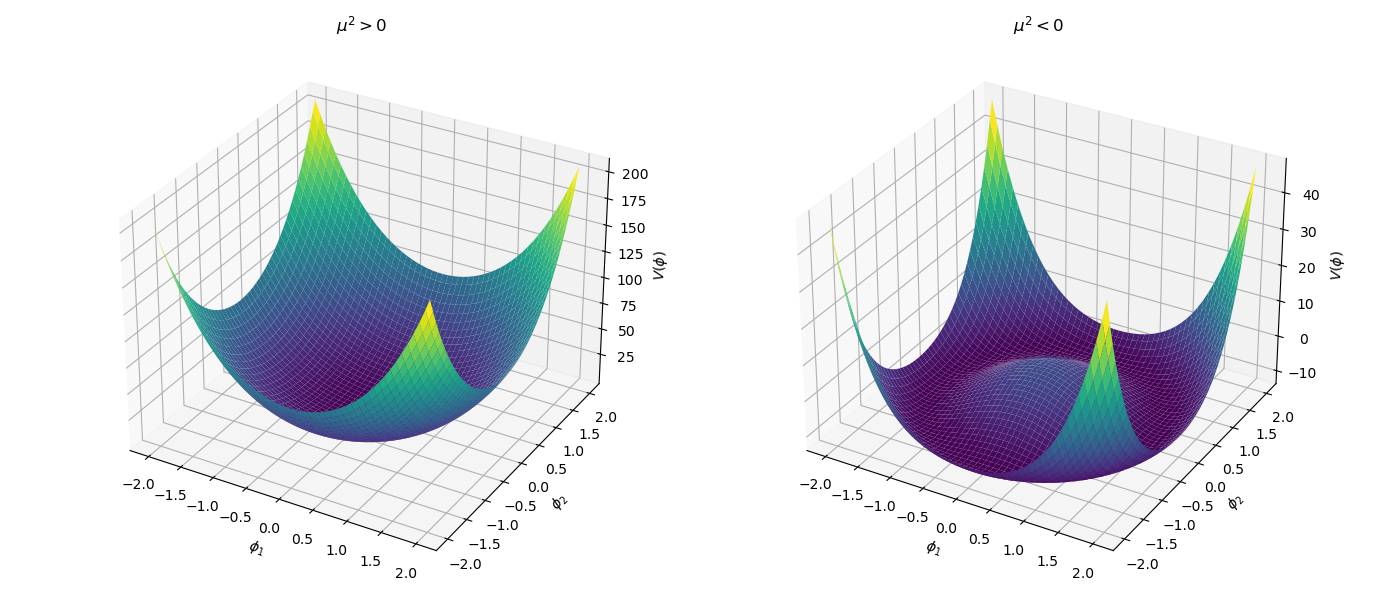
\includegraphics[width=1.0\textwidth]{images/Higgs_Potential.png}
    \caption{Visual representation of the Higgs potential (with $\lambda = 2$) for positive $\mu^2 = 10$ (left) and 
    negative $\mu^2 = -10$ (right).}
    \label{fig:Higgs_Potential}
\end{figure}

In the case where $\mu^2 < 0$, this potential requires a physical choice for the minimum (vacuum) state which 
explicitly breaks the rotational symmetry in the $(\phi_1, \phi_2)$ plane. The minimum energy of the system, also 
known as the vacuum expectation value (or VEV), is at $v = \sqrt{\frac{-\mu^2}{\lambda}}$ for such a theory. \par

In the Standard Model we require the scalar field to be a complex $SU(2)$ doublet

\begin{equation}
\phi = 
\begin{pmatrix} \phi^+  \\ \phi^0 \end{pmatrix}
= \frac{1}{\sqrt{2}}
\begin{pmatrix} \phi_1 + i\phi_2 \\ \phi_3 + i\phi_4 \end{pmatrix}
\end{equation}

which given $\mu^2 < 0$ has an infinite number of minima where $\phi^\dagger\phi = \frac{v^2}{2}$. For physical 
reasons related to the absence of photon mass, the vacuum expectation value is only non-zero for the $\phi^0$ 
component of the doublet, such that we can expand the field around this minimum as

\begin{equation}
\phi(x) = \frac{1}{\sqrt{2}}
\begin{pmatrix} 0 \\ v + h(x) \end{pmatrix}
\end{equation}

This field description is in unitary gague where $h(x)$ directly represents the physical Higgs field. An equivalent, 
but more general description of this expansion around the VEV can be done by including an additional perturbing 
field around the minimum of $\phi^+$ and then removing non-physical fields via gauge transformation afterwards. 
In the end, the symmetry breaking of this new scalar potential immediately results in the introduction of weak
boson mass terms in the Lagrangian as well as an entirely new particle: the Higgs boson.

\subsection{Particle Masses and Higgs Interactions}

The new terms can be seen directly if we expand the kinetic term of the scalar field Lagrangian around the VEV as

\begin{equation}
\begin{aligned}
(D_{\mu}\phi)^{\dagger}(D^{\mu}\phi) =& \frac{1}{2}(\partial_{\mu}h)(\partial^{\mu}h) + 
\frac{1}{8}g_W^2(W_{\mu}^{(1)} + iW_{\mu}^{(2)})(W^{(1)\mu} - iW^{(2)\mu})(v+h)^2 + \\
&\frac{1}{8}(g_WW_{\mu}^{(3)} - g'B_{\mu})(g_WW^{(3)\mu} - g'B^{\mu})(v+h)^2 \\
=&\frac{1}{2}(\partial_{\mu}h)(\partial^{\mu}h) + \frac{1}{4}g_W^2W_{\mu}^-W^{+\mu}(v+h)^2 + 
\frac{1}{4}(g_W^2+g'^2)Z_{\mu}Z^{\mu}(v+h)^2
\end{aligned}
\end{equation}

where we have written the physical particles as combinations of the underlying fields 
$W^{\pm} = \frac{1}{\sqrt{2}}(W^{(1)} \mp iW^{(2)})$ and 
$Z = (g^2_W + g'^2)^{-\frac{1}{2}}(g_WW^{(3)} - g'B)$. In this expression,  the $v^2$ terms represent 
the weak boson masses (i.e. self-interaction terms) while $vh$ and $h^2$ terms describe the couplings 
(i.e. interaction strengths) between two weak bosons and one or two Higgs bosons respectively. The masses 
can be read directly from the Lagrangian as $m_W = \frac{1}{2}g_Wv$ and 
$m_Z = \frac{1}{2}v\sqrt{g^2_W + g'^2}$. As expected, there is no mass term for the photon, which means 
it does not interact with the Higgs boson. Requiring orthogonality to the $Z$, we can see that the photon is 
represented as $A = (g^2_W + g'^2)^{-\frac{1}{2}}(g'W^{(3)} + g_WB)$. Repeating the above expansion 
with the potential term of the scalar field Lagrangian results in 

\begin{equation}
V(\phi) = \frac{1}{2}\mu^2(v+h)^2 + \frac{1}{4}\lambda(v+h)^4 = 
\lambda v^2h^2 + \lambda vh^3 + \frac{1}{4}\lambda h^4 - \frac{1}{4}\lambda v^4
\end{equation}

where $h^2$ terms define the Higgs mass $m_H = \sqrt{2\lambda}v$ and $h^3$ and $h^4$ terms the 
self-couplings between 3 and 4 Higgs bosons respectively. \par

These new additions to the Standard Model Lagrangian bring out the missing mass terms for weak bosons 
via the introduction of a massive scalar boson: the Higgs. Fermions on the other hand, are still unaccounted 
for.Thankfully, the Higgs field allows for the introduction of gauge invariant fermion mass terms which 
complete the picture. In particular these take the form of 
$-g_f(\bar{\psi_L}\phi\psi_R + \bar{\psi_R}\phi^{\dagger}\psi_L)$ and 
$g_f(\bar{\psi_L}\phi_C\psi_R + \bar{\psi_R}\phi_C^{\dagger}\psi_L)$ where $\phi_C = -i\sigma_2\phi^*$ 
is the conjugate Higgs doublet. Both of these expressions satisfy the $SU(2)_L \times U(1)_Y$ symmetry of 
the Standard Model as required.Since the VEV is only non-zero for the lower component of the scalar 
$SU(2)$ doublet (i.e. $\phi^0$), the first expression generates the charged lepton and down-type quark 
terms while the second is responsible for the up-type quarks

\begin{equation}
\mathcal{L}_f = -\frac{g_f}{\sqrt{2}}v(\bar{f_L}f_R + \bar{f_R}f_L) - 
\frac{g_f}{\sqrt{2}}h(\bar{f_L}f_R + \bar{f_R}f_L)
\end{equation}

Aside from neutrinos, which represent a bigger mystery due to their apparent fixed left-handedness, this 
Lagrangian describes the masses and Higgs interactions of all fermions. The Yukawa coupling 
$g_f$ determines the coupling strength between a particular fermion and the Higgs and is not fixed by 
theory. Various BSM models predict modifications to the Yukawa couplings of fermions which could have a 
significant impact on the mass generation mechanism of the Standard Model 
\cite{gunion-2hdm, carena-mssm}. These deviations are measurable via changes in interaction rates 
between the Higgs and different fermions, which constitutes the main focus of my thesis.

\subsection{Why the Higgs is Interesting}

While the Standard Model is mathematically robust and broadly experimentally tested, there are many open 
questions about elements of its Lagrangian. It has 19 free parameters that are not fixed by theoretical 
predictions. Of these, 9 are related to the Yukawa couplings, 4 to the CKM matrix (3 angles + 1 phase), 3 are 
coupling strengths, 2 are related to the Higgs mass and VEV and 1 specifies CP violation in QCD. An additional 7 
free parameters are related to neutrinos (3 masses and 4 oscillation angles). Thus, a grand total of 11 free 
parameters are related to the Higgs boson and the Higgs mechanism, which represents the newest and least 
understood piece of the Standard Model overall. At the forefront of these are the Yukawa couplings. Some 
(such as the top Yukawa) are relatively well understood, leading us to the expectation that 
$g_f = \sqrt{2}\frac{m_f}{v}$. Deviations from this expectation could provide a window into physics beyond 
the Standard Model, potentially leading us a deeper understanding of the structure of the theory itself.  \par

As it stands our theory is missing descriptions of gravity, dark matter and neutrino masses as well as answers 
to questions related to the existence of exactly three generations of fermions with different masses, the origins 
of this mass hierarchy, particle-antiparticle asymmetry and so much more. There are also still fundamental 
questions about the Higgs mass itself, which is predicted to be much larger than observed due to quantum 
corrections $\delta m_H^2 \sim \frac{\Lambda^2}{16\pi^2}$ \footnote{Here $\Lambda = 10^{19}\ GeV$, which 
corresponds to the Planck scale} that require unnatural fine-tuning to cancel, leading to what is called the 
"naturalness problem" \cite{susskind-naturalness}. Thus the study of the Higgs boson and its interactions 
with other particles are crucial pieces in expanding our understanding of the Standard Model and answering 
these open questions. In particular, my work is focused on the charm Yukawa coupling which is still not well 
understood.  As the heaviest second generation quark, the charm quark represents the best way of moving 
towards a unified understanding of how the Higgs interacts with lighter particles.In practice this requires a 
mechanism to produce Higgs bosons, which is best done in high energy particle colliders as will be explored 
in the following section.

\section{Collider Physics}

The usefulness of particle colliders comes from their ability to facilitate high energy particle interactions in 
a vacuum (both literally and figuratively). The higher the center of mass energy in these collisions, the more 
interactions are accessible for study since the collision energy needs to at least match the rest mass of the 
interaction products. The colliding particles in question are either hadrons (usually protons or anti-protons) 
or leptons (i.e. electrons). Electrons are easier to accelerate and provide cleaner signatures since they are 
fundamental particles themselves, but they lose energy rapidly due to bremsstrahlung and do not allow for 
probing QCD interactions. Because of this, the most versatile colliders tend to be hadron beam colliders, 
which simultaneously accelerate two beams of hadrons to maximize collision energy. This category includes 
the Large Hadron Collider (LHC): a circular proton-proton collider and one of the core tools of my research. 
While the LHC will be discussed in more detail later, the following section is intended to give a general 
overview of some of the important theoretical aspects of hadron colliders as well as introduce some 
terminology in preparation.

\subsection{Basics of Hadron Collisions}

The center of mass energy of a beam collider $s = (\Sigma^2_{i=1}E_i)^2 - (\Sigma^2_{i=1}\mathbf{p}_i)^2$ is 
one of its most important characteristics. In hadron colliders, this does not correspond directly to the collision 
energy since "hard scatter"\footnote{In this context, "hard" refers to processes that occur at high enough energies 
to break apart the colliding hadrons while "soft" generally refers to lower energy radiation.} collisions occur between 
so called "partons" (i.e. quarks and gluons) that make up each hadron rather than the hadrons themselves. This has 
two tangible consequences. The first is that we need to account for the unknown parton momentum fraction in 
each collision. We do this via so-called parton density functions (PDFs) that get factored into our calculations. As 
such, the center of mass energy acts as an upper bound for the parton collision energy, which determines 
accessible final states. Secondly, event signatures are much messier in hadronic collisions compared to leptonic 
ones due to color confinement in QCD. In practice this is due to the fact that parton collisions have an impact on 
other partons in their respective hadronic bound states. \par

Aside from $\sqrt{s}$, the other important quantity associated with the design of the 
collider is the instantaneous luminosity $L = \frac{1}{\sigma}\frac{dN}{dt}$ which relates the cross section to 
the event rate. Integrating this quantity over time gives the total integrated Luminosity $L_{int}$ which is a 
measure of the total number of collision events recorded over time that is independent of the specific 
physical process under consideration.Due to the nature of beam accelerators there are generally multiple 
collisions happening at any given time of which many are uninteresting. These auxiliary interactions are called 
"pile-up" and need to be filtered out from any interesting "hard scatter" collisions observed. \par

After producing particle collisions, we require a detector to record the signatures contained in the final state.
In essence, particle detectors are large and elaborate counting devices built to answer the question of how many 
times a particular process of interest is observed relative to expectations based on theory. To quantify this we 
use the cross section $sigma$, which represents the probability that a specific process will take place. Given an 
interaction $pp \rightarrow X$ the total cross section related to the number of measured events of process $X$ 
and the luminosity is a combination of all possible parton pair cross sections. This combination is dependent on 
the proton PDFs (parton distribution functions) $f_{q/g}(x)$ which describe the probability of finding a 
particular quark flavor or gluon with a specific fraction $x$ of the total proton momentum. Putting this together 
results in a rather complicated combination of the soft long-range dynamics described in the proton PDFs and 
the hard scatter parton collision in which we're ultimately interested. Thankfully, the factorization theorem within 
QCD \cite{collins-qcd-factorization} allows us to separate these two processes since the hard scatter collision 
can be treated perturbatively, leading to 

\begin{equation}
d\sigma_{pp \rightarrow X} \sim 
\Sigma_{a,b} \int dx_{p1} f_{a}(x_{p1}, \mu_F) \int dx_{p2} f_{b}(x_{p2}, \mu_F) d\sigma_{ab \rightarrow X}
\label{eqn:parton-cross-section}
\end{equation}

Here $\mu_F$ is a parameter called the factorization scale, corresponding to the energy cutoff where we can 
perform these perturbative calculations\footnote{The underlying reason for this is the "running" of the QCD 
coupling, which causes it to become small at high energies (in contrast to QED)}. While the cross sections 
$\sigma_{ab \rightarrow X}$ can be calculated via QCD, the proton PDFs need to be determined empirically via 
experiments \cite{bailey-proton-pdfs}.

\subsection{Final States and Hadronization}

The aforementioned process $pp \rightarrow X$ serves as an umbrella for all of the physics happening at the 
stage of the hard scatter collision producing a collection of particles denoted $X$. These dynamics are generally 
well understood mathematically and calculable using QCD techniques. However, due to the short lifetimes $\tau$ 
of many particles produced in these environments, $X$ does not generally correspond to the final state particles 
observed in a detector. If we care about a particular final state, we use the branching ratio to describe the fraction 
of times a particular decay mode $j$ occurs as $BR(j) = \frac{\Gamma_j}{\Gamma}$ where 
$\Gamma = \frac{1}{\tau}$ is the total decay rate of our particle of interest and is related to its overall lifetime. \par

One additional complexity comes from color confinement in QCD, which forces individual partons into bound states. 
This imposes extra constraints on the possible final states of any given collision event through a process called 
hadronization. This process ensures partons involved in high-energy collisions end up in new bound states via the 
production of new quark-antiquark pairs. QCD factorization again allows us to separate hadronization from the 
underlying hard scatter event. While it is not entirely understood, it originates in the linear potential 
$V(\mathbf{r}) \sim \kappa\mathbf{r}$ (where $\kappa \sim 1\ GeV/fm$) experienced by quarks or gluons outside 
of bound states. As the distance between bound quarks increases due to the momentum imparted by a collision 
event, it eventually becomes energetically favorable to form new bound states via the spontaneous creation of new 
quark-antiquark pairs. This process continues until the partons within each bound state have a low enough energy 
to remain bound, thereby creating a number of new hadrons. In practice, these hadrons manifest as collimated 
sprays of particles originating from a common point, which are called particle jets. These structure play a central role 
in the identification of various event signatures, including Higgs to charm decays and will be discussed in detail 
in a later section.

\subsection{Monte Carlo Simulations}

Hadron collisions are very high dimensional events due to the immense number of final state particles created 
in the combination of "hard scatter" collision, pile-up and initial- and final state radiation (ISR and FSR)
\footnote{ISR and FSR corresponds to low energy QCD and EM radiation happening before or after the "hard scatter" 
collision respectively}. In order to have a good understanding of their structure in a particle detector based on 
theoretical expectations, we need to make use of Monte Carlo techniques to generate simulated collision events. 
These simulations are based on existing knowledge of (and expectations from) Standard Model physics or any 
other underlying theory to be tested. Monte Carlo event generation occurs in multiple steps (thanks to QCD 
factorization) and uses random sampling to generate a realistic distribution of events that can be compared 
against data to test our underlying theory. \par

The core of these generators concerns the cross sections of "hard scatter" parton collisions 
(\ref{eqn:parton-cross-section}), which are not analytically tractable. Using numerical techniques these can be 
estimated to some precision, usually leading order (LO), next-to-leading order (NLO) or next-to-next-to leading 
order (NNLO) in QCD. While these calculations are exact at infinite order, there are theoretical uncertainties 
associated with cutting them off at finite precision, which represents a trade-off due to high compute 
requirements. Some of these higher order corrections are approximated via parton showering algorithms which 
add additional parton contributions via ISR and FSR to the "hard scatter" collision. Once all of the final state 
partons are generated, hadronization algorithms are used to develop the final structure of the primary collision. 
These algorithms are based on phenomenological models derived from lattice QCD and are not exact. Finally 
the so called "underlying event" is generated which is not related to the primary collision but is necessary to 
model pile-up. All of the final state particles are passed through a detector simulation to approximate the 
expected readout. A graphical summary of this pipeline is given in figure \ref{fig:Monte_Carlo}.

%https://link.springer.com/chapter/10.1007/978-3-030-65380-4_2
\begin{figure}
\centering
    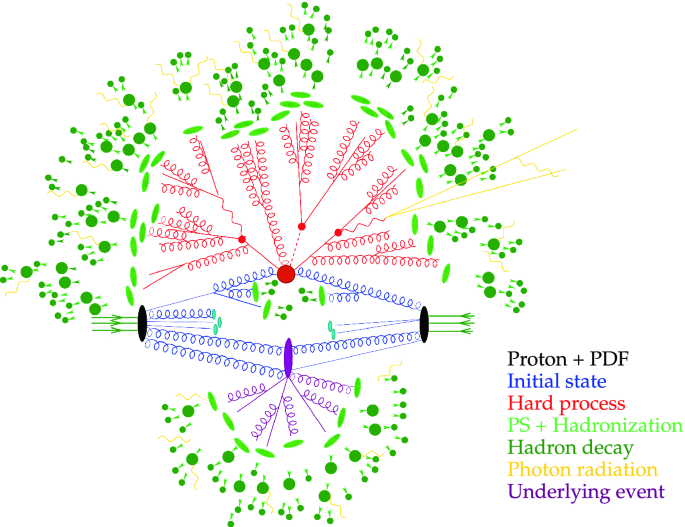
\includegraphics[width=0.8\textwidth]{images/Monte_Carlo.png}
    \caption{Visual representation of a $t\bar{t}$ production event as simulated by a Monte Carlo generator).}
    \label{fig:Monte_Carlo}
\end{figure}

\subsection{Higgs Production and Decay}

Among the many possible products of hadron collisions are Higgs bosons, which are the objects of study of my 
research. Overall, there are 4 common modes of Higgs production in hadron collisions summarized in figure 
\ref{fig:Higgs_Production}: gluon-gluon fusion (ggF),  vector boson fusion (VBF), associated production with a 
vector boson or Higgs strahlung ($VH$) and associated production with a top\footnote{Top quark pairs are by far 
the most common in this mode due to the large top Yukawa coupling, but other quark pairs contribute as well} quark 
pair ($t\bar{t}H$). Each mode allows us to study the Higgs boson, but some are easier to identify than others in 
practice. Finding Higgs bosons is generally simpler if there are other unique signatures present in the collision event.
Because of these differences as well as differences in frequencies for each mode, studies are ususally performed 
separately by production mode and combined afterwards. My research focuses on the $VH$ mode because it is 
the easiest to identify in the context of Higgs to charm decays, as will be explained in more detail in a later 
chapter. \par

%https://cds.cern.ch/record/2243593/plots
\begin{figure}
\centering
    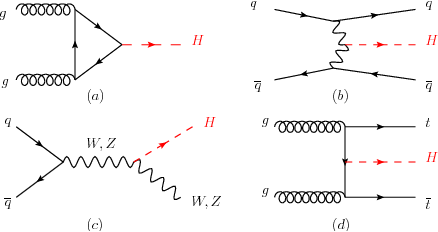
\includegraphics[width=0.6\textwidth]{images/Higgs_Production.png}
    \caption{Feynman diagrams for the most common Higgs production modes: a) ggF, b) VBF, c) $VH$, 
    d) $t\bar{t}H$.}
    \label{fig:Higgs_Production}
\end{figure}

The Higgs is a very short lived particle with a predicted mean lifetime of $1.56 \times 10^{-22}\ s$, which is short 
enough that at energies relevant for collider physics it does not travel a measurable distance between its production 
and decay. As such, studying the Higgs boson requires identifying its final decay products. This is also the best avenue 
to measuring many of the Yukawa couplings, such as the charm Yukawa since the fraction of Higgs bosons produced 
in association with a charm quark pair is vanishingly small. Instead we look at the Higgs decaying to a pair of charm 
quarks, which is one of its main decay modes summarized in table \ref{table-higgs-decay}. \par

Higgs to charm is a difficult measurement to make for many reasons,including the difficulty of producing and 
isolating events containing Higgs bosons, the relatively small $H \rightarrow c\bar{c}$ branching ratio as well as the 
challenge in identifying charm quarks more generally. All of these challenges start with the hardware used to 
accomplish all of this: the LHC and the ATLAS detector which will be the subject of the next chapter.

\begin{table}
\begin{center}
\caption{Summary of Higgs decay modes with associated branching ratios based on Standard Model predictions \cite{atlas-higgs-decay}.}
\label{table-higgs-decay}
\begin{tabular}{|c c|} 
 \hline
 Decay channel & Branching ratio [\%] \\ [0.5ex] 
 \hline
 $H \rightarrow b\bar{b}$ & $57.5 \pm 1.9$ \\ 
 $H \rightarrow W^+W^-$ & $21.6 \pm 0.9$ \\ 
 $H \rightarrow gg$ & $8.56 \pm 0.86$ \\ 
 $H \rightarrow \tau^+\tau^-$ & $6.30 \pm 0.36$ \\ 
 $H \rightarrow c\bar{c}$ & $2.90 \pm 0.35$ \\
 $H \rightarrow ZZ$ & $2.67 \pm 0.11$ \\
 $H \rightarrow \gamma\gamma$ & $0.228 \pm 0.011$ \\
 $H \rightarrow Z\gamma$ & $0.155 \pm 0.014$ \\
 $H \rightarrow \mu^+\mu^-$ & $0.022 \pm 0.001$ \\
 \hline
\end{tabular}
\end{center}
\end{table}